\documentclass[tikz, border= 10pt]{standalone}
\usepackage{pgfplots}
\pgfplotsset{compat = 1.18, width = 10cm}
\usetikzlibrary{shapes.misc}
\usetikzlibrary{patterns}
\usetikzlibrary{positioning}
\usepgfplotslibrary{fillbetween, groupplots}

\tikzset{cross/.style={cross out, draw=black, minimum size=2*(#1-\pgflinewidth), inner sep=0pt, outer sep=0pt},
%default radius will be 1pt. 
cross/.default={5pt}}

\begin{document}
%Q1
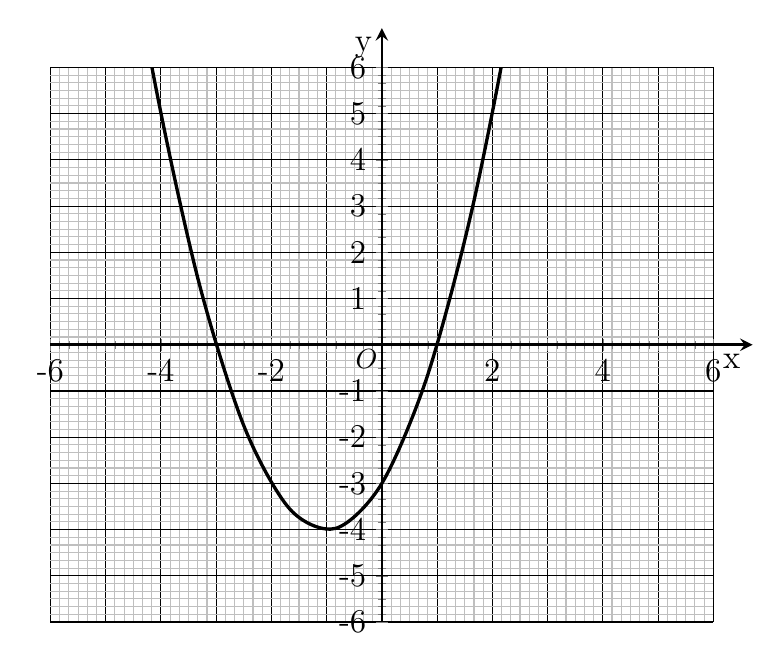
\begin{tikzpicture}
\begin{axis}
[
axis lines=middle,
axis line style = {line width = 1pt, shorten >=-5mm },
xlabel = x,
ylabel = y,
xlabel style = {anchor = north west, font = \large},
ylabel style = {anchor = south east, font = \large},
ymajorgrids=true,
xmajorgrids=true,
xminorgrids = true,
yminorgrids = true,
minor tick num=5,
minor grid style = {gray!50},
grid style={black!100},
xmin=-6,
xmax=6,
ymin=-6,
ymax=6,
xtick={-6,-5,...,6},
xticklabels = {-6, {}, -4, {}, -2, {}, {}, {}, {2}, {} ,{4}, {}, {6} },
xticklabel style = {font = \large},
ytick={-6,-5,...,6},
yticklabel style = {font = \large},
tick label style={/pgf/number format/assume math mode=true},
]
\node[anchor = north east] at (axis cs: 0.1,0.1) {$O$};
\addplot[color =black,line width = 1.2pt, domain = -10:10, name path = A, smooth]{x*x + 2*x - 3};

    \end{axis}
\end{tikzpicture}

%Q2
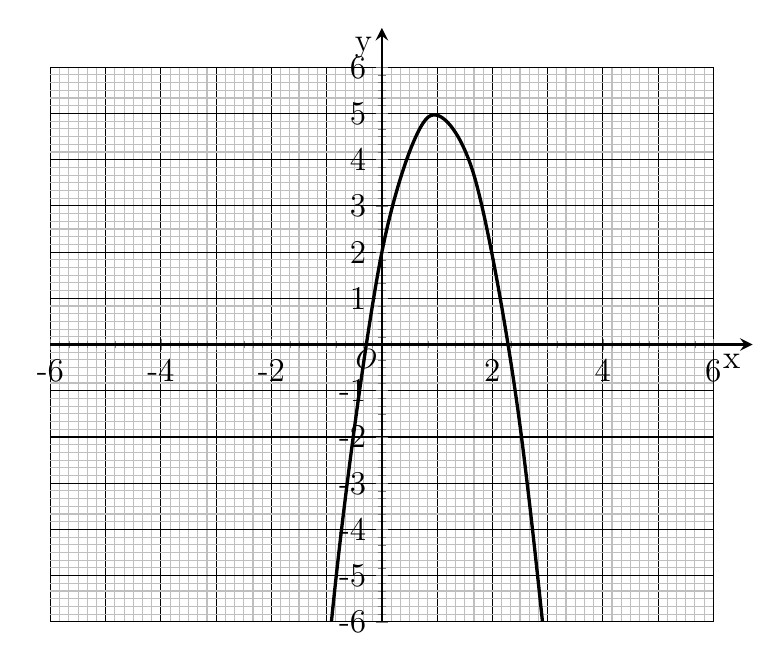
\begin{tikzpicture}
\begin{axis}
[
axis lines=middle,
axis line style = {line width = 1pt, shorten >=-5mm },
xlabel = x,
ylabel = y,
xlabel style = {anchor = north west, font = \large},
ylabel style = {anchor = south east, font = \large},
ymajorgrids=true,
xmajorgrids=true,
xminorgrids = true,
yminorgrids = true,
minor tick num=5,
minor grid style = {gray!50},
grid style={black!100},
xmin=-6,
xmax=6,
ymin=-6,
ymax=6,
xtick={-6,-5,...,6},
xticklabels = {-6, {}, -4, {}, -2, {}, {}, {}, {2}, {} ,{4}, {}, {6} },
xticklabel style = {font = \large},
ytick={-6,-5,...,6},
yticklabel style = {font = \large},
tick label style={/pgf/number format/assume math mode=true},
]
\node[anchor = north east] at (axis cs: 0.1,0.1) {$O$};
\addplot[color =black,line width = 1.2pt, domain = -10:10, name path = A, smooth]{-3*x*x + 6*x +2};

    \end{axis}
\end{tikzpicture}

%Q3
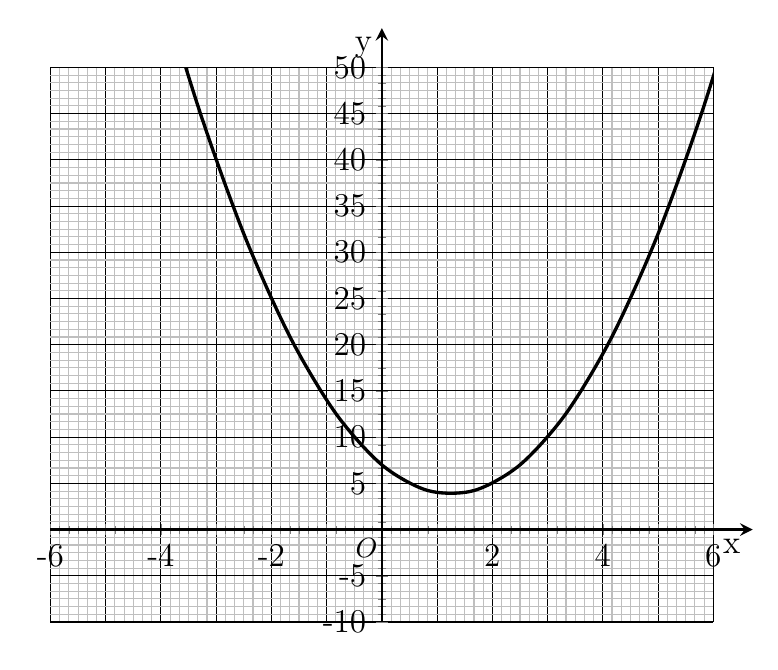
\begin{tikzpicture}
\begin{axis}
[
axis lines=middle,
axis line style = {line width = 1pt, shorten >=-5mm },
xlabel = x,
ylabel = y,
xlabel style = {anchor = north west, font = \large},
ylabel style = {anchor = south east, font = \large},
ymajorgrids=true,
xmajorgrids=true,
xminorgrids = true,
yminorgrids = true,
minor tick num=5,
minor grid style = {gray!50},
grid style={black!100},
xmin=-6,
xmax=6,
ymin=-10,
ymax=50,
xtick={-6,-5,...,6},
xticklabels = {-6, {}, -4, {}, -2, {}, {}, {}, {2}, {} ,{4}, {}, {6} },
xticklabel style = {font = \large},
ytick={-10,-5,...,50},
yticklabel style = {font = \large},
tick label style={/pgf/number format/assume math mode=true},
]
\node[anchor = north east] at (axis cs: 0.1,0.1) {$O$};
\addplot[color =black,line width = 1.2pt, domain = -10:10, name path = A, smooth]{2*x*x - 5*x + 7};

    \end{axis}
\end{tikzpicture}

%Q4
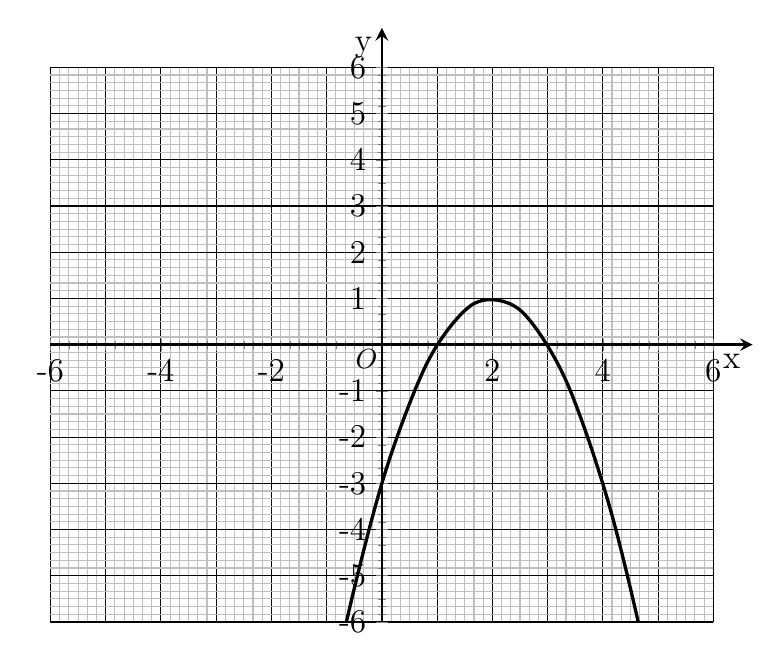
\begin{tikzpicture}
\begin{axis}
[
axis lines=middle,
axis line style = {line width = 1pt, shorten >=-5mm },
xlabel = x,
ylabel = y,
xlabel style = {anchor = north west, font = \large},
ylabel style = {anchor = south east, font = \large},
ymajorgrids=true,
xmajorgrids=true,
xminorgrids = true,
yminorgrids = true,
minor tick num=5,
minor grid style = {gray!50},
grid style={black!100},
xmin=-6,
xmax=6,
ymin=-6,
ymax=6,
xtick={-6,-5,...,6},
xticklabels = {-6, {}, -4, {}, -2, {}, {}, {}, {2}, {} ,{4}, {}, {6} },
xticklabel style = {font = \large},
ytick={-6,-5,...,6},
yticklabel style = {font = \large},
tick label style={/pgf/number format/assume math mode=true},
]
\node[anchor = north east] at (axis cs: 0.1,0.1) {$O$};
\addplot[color =black,line width = 1.2pt, domain = -10:10, name path = A, smooth]{-x*x + 4*x - 3};

    \end{axis}
\end{tikzpicture}

%Q5
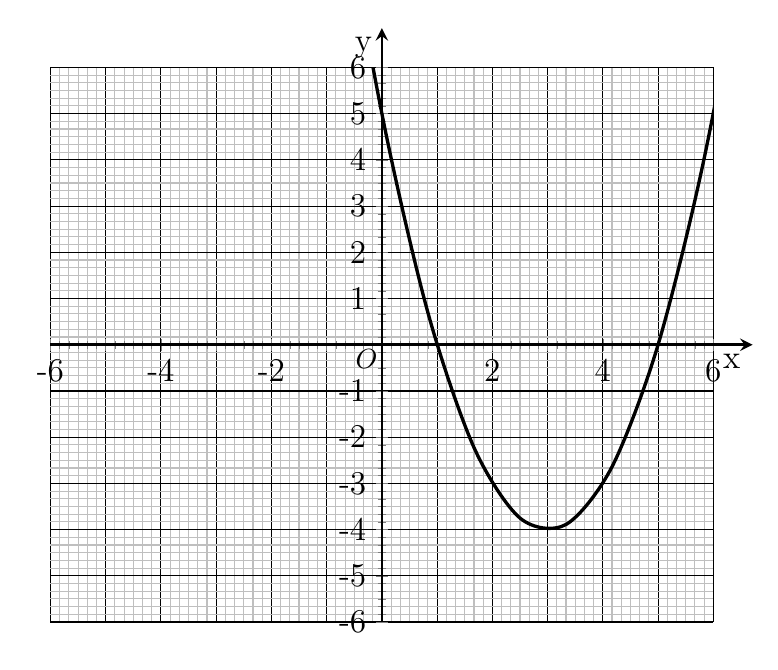
\begin{tikzpicture}
\begin{axis}
[
axis lines=middle,
axis line style = {line width = 1pt, shorten >=-5mm },
xlabel = x,
ylabel = y,
xlabel style = {anchor = north west, font = \large},
ylabel style = {anchor = south east, font = \large},
ymajorgrids=true,
xmajorgrids=true,
xminorgrids = true,
yminorgrids = true,
minor tick num=5,
minor grid style = {gray!50},
grid style={black!100},
xmin=-6,
xmax=6,
ymin=-6,
ymax=6,
xtick={-6,-5,...,6},
xticklabels = {-6, {}, -4, {}, -2, {}, {}, {}, {2}, {} ,{4}, {}, {6} },
xticklabel style = {font = \large},
ytick={-6,-5,...,6},
yticklabel style = {font = \large},
tick label style={/pgf/number format/assume math mode=true},
]
\node[anchor = north east] at (axis cs: 0.1,0.1) {$O$};
\addplot[color =black,line width = 1.2pt, domain = -10:10, name path = A, smooth]{x*x - 6*x + 5};

    \end{axis}
\end{tikzpicture}

%Q6
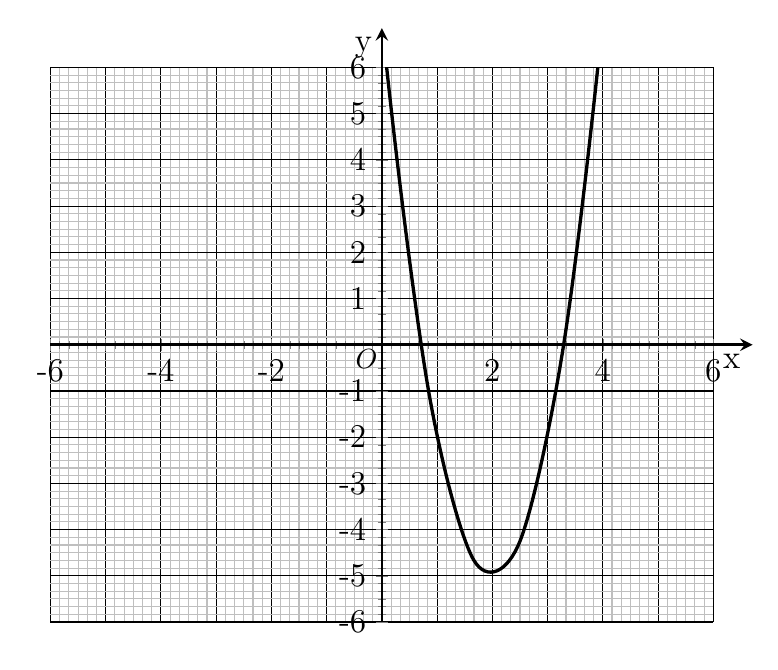
\begin{tikzpicture}
\begin{axis}
[
axis lines=middle,
axis line style = {line width = 1pt, shorten >=-5mm },
xlabel = x,
ylabel = y,
xlabel style = {anchor = north west, font = \large},
ylabel style = {anchor = south east, font = \large},
ymajorgrids=true,
xmajorgrids=true,
xminorgrids = true,
yminorgrids = true,
minor tick num=5,
minor grid style = {gray!50},
grid style={black!100},
xmin=-6,
xmax=6,
ymin=-6,
ymax=6,
xtick={-6,-5,...,6},
xticklabels = {-6, {}, -4, {}, -2, {}, {}, {}, {2}, {} ,{4}, {}, {6} },
xticklabel style = {font = \large},
ytick={-6,-5,...,6},
yticklabel style = {font = \large},
tick label style={/pgf/number format/assume math mode=true},
]
\node[anchor = north east] at (axis cs: 0.1,0.1) {$O$};
\addplot[color =black,line width = 1.2pt, domain = -10:10, name path = A, smooth]{3*x*x - 12*x + 7};

    \end{axis}
\end{tikzpicture}

%Q7
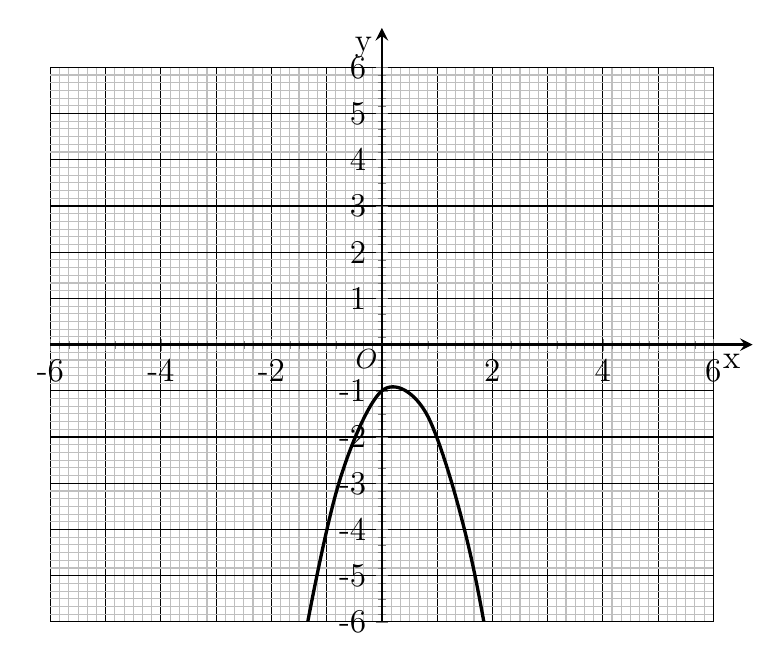
\begin{tikzpicture}
\begin{axis}
[
axis lines=middle,
axis line style = {line width = 1pt, shorten >=-5mm },
xlabel = x,
ylabel = y,
xlabel style = {anchor = north west, font = \large},
ylabel style = {anchor = south east, font = \large},
ymajorgrids=true,
xmajorgrids=true,
xminorgrids = true,
yminorgrids = true,
minor tick num=5,
minor grid style = {gray!50},
grid style={black!100},
xmin=-6,
xmax=6,
ymin=-6,
ymax=6,
xtick={-6,-5,...,6},
xticklabels = {-6, {}, -4, {}, -2, {}, {}, {}, {2}, {} ,{4}, {}, {6} },
xticklabel style = {font = \large},
ytick={-6,-5,...,6},
yticklabel style = {font = \large},
tick label style={/pgf/number format/assume math mode=true},
]
\node[anchor = north east] at (axis cs: 0.1,0.1) {$O$};
\addplot[color =black,line width = 1.2pt, domain = -10:10, name path = A, smooth]{-2*x*x + x - 1};

    \end{axis}
\end{tikzpicture}

%Q8
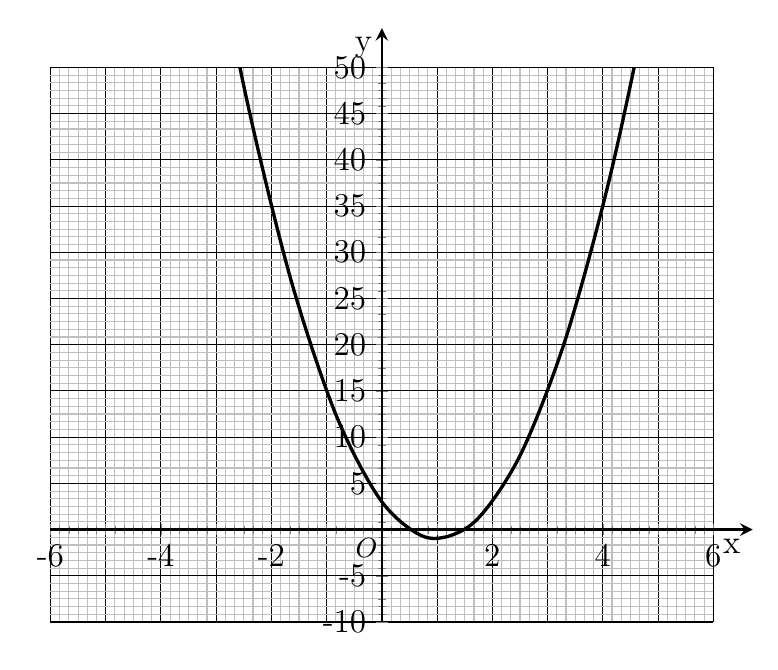
\begin{tikzpicture}
\begin{axis}
[
axis lines=middle,
axis line style = {line width = 1pt, shorten >=-5mm },
xlabel = x,
ylabel = y,
xlabel style = {anchor = north west, font = \large},
ylabel style = {anchor = south east, font = \large},
ymajorgrids=true,
xmajorgrids=true,
xminorgrids = true,
yminorgrids = true,
minor tick num=5,
minor grid style = {gray!50},
grid style={black!100},
xmin=-6,
xmax=6,
ymin=-10,
ymax=50,
xtick={-6,-5,...,6},
xticklabels = {-6, {}, -4, {}, -2, {}, {}, {}, {2}, {} ,{4}, {}, {6} },
xticklabel style = {font = \large},
ytick={-10,-5,...,50},
yticklabel style = {font = \large},
tick label style={/pgf/number format/assume math mode=true},
]
\node[anchor = north east] at (axis cs: 0.1,0.1) {$O$};
\addplot[color =black,line width = 1.2pt, domain = -10:10, name path = A, smooth]{4*x*x - 8*x + 3};

    \end{axis}
\end{tikzpicture}

%Q9
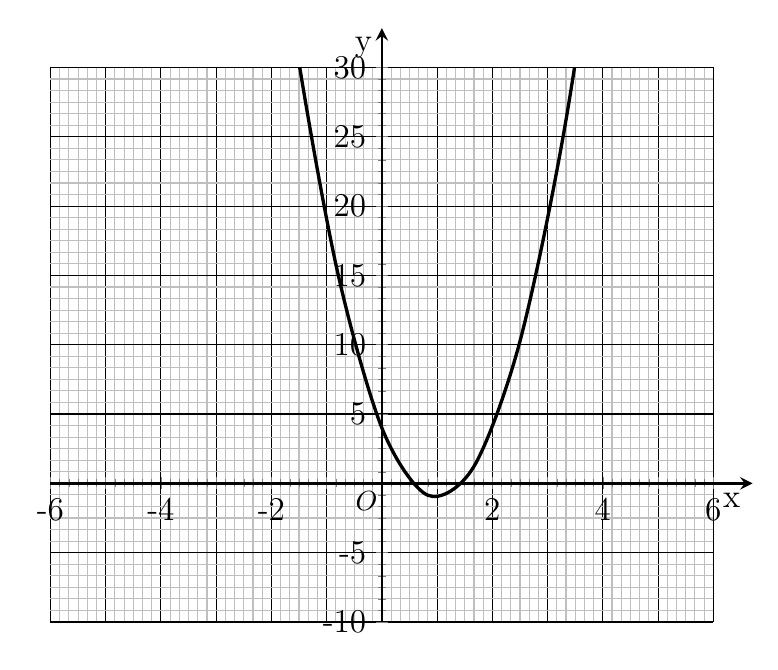
\begin{tikzpicture}
\begin{axis}
[
axis lines=middle,
axis line style = {line width = 1pt, shorten >=-5mm },
xlabel = x,
ylabel = y,
xlabel style = {anchor = north west, font = \large},
ylabel style = {anchor = south east, font = \large},
ymajorgrids=true,
xmajorgrids=true,
xminorgrids = true,
yminorgrids = true,
minor tick num=5,
minor grid style = {gray!50},
grid style={black!100},
xmin=-6,
xmax=6,
ymin=-10,
ymax=30,
xtick={-6,-5,...,6},
xticklabels = {-6, {}, -4, {}, -2, {}, {}, {}, {2}, {} ,{4}, {}, {6} },
xticklabel style = {font = \large},
ytick={-10,-5,...,30},
yticklabel style = {font = \large},
tick label style={/pgf/number format/assume math mode=true},
]
\node[anchor = north east] at (axis cs: 0.1,0.1) {$O$};
\addplot[color =black,line width = 1.2pt, domain = -10:10, name path = A, smooth]{5*x*x - 10*x + 4};

    \end{axis}
\end{tikzpicture}

%Q10
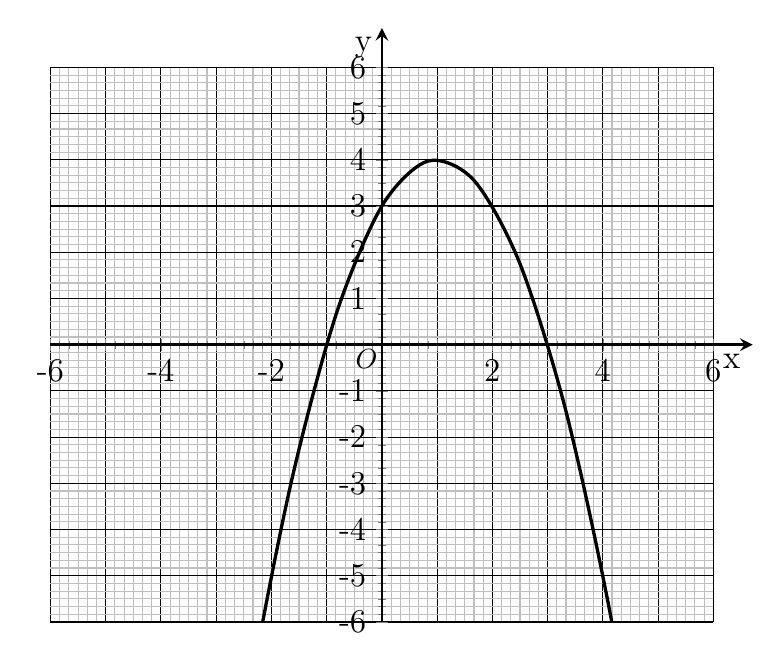
\begin{tikzpicture}
\begin{axis}
[
axis lines=middle,
axis line style = {line width = 1pt, shorten >=-5mm },
xlabel = x,
ylabel = y,
xlabel style = {anchor = north west, font = \large},
ylabel style = {anchor = south east, font = \large},
ymajorgrids=true,
xmajorgrids=true,
xminorgrids = true,
yminorgrids = true,
minor tick num=5,
minor grid style = {gray!50},
grid style={black!100},
xmin=-6,
xmax=6,
ymin=-6,
ymax=6,
xtick={-6,-5,...,6},
xticklabels = {-6, {}, -4, {}, -2, {}, {}, {}, {2}, {} ,{4}, {}, {6} },
xticklabel style = {font = \large},
ytick={-6,-5,...,6},
yticklabel style = {font = \large},
tick label style={/pgf/number format/assume math mode=true},
]
\node[anchor = north east] at (axis cs: 0.1,0.1) {$O$};
\addplot[color =black,line width = 1.2pt, domain = -10:10, name path = A, smooth]{-x*x + 2*x +3};

    \end{axis}
\end{tikzpicture}


\end{document}